\documentclass[10pt]{beamer}
\usepackage{tikz}
\usepackage[ruled]{algorithm2e}
\usepackage{bbm}

\mode<presentation> {
    \usetheme{Madrid}
}

\usepackage{babel}
\usepackage[utf8]{inputenc}
\usepackage{graphicx} 
\usepackage{booktabs} 


\date{\today}

\AtBeginSection[]
{
\begin{frame}
\frametitle{Contents}
\tableofcontents[currentsection]
\end{frame}
}


\title[Computational Optimal Transportation]
{Computational Optimal Transportation} 

\author[Michael Rawson]{
Michael Rawson} 

\newcommand{\R}{{\mathbb{R}}}
\newcommand{\C}{{\mathcal{C}}}
\newcommand{\E}{{\mathbb{E}}}
\newcommand{\F}{{\mathcal{F}}}
\newcommand{\A}{{\mathcal{A}}}
\newcommand{\HH}{{\mathcal{H}}}
\newcommand{\M}{{\mathcal{M}}}
\newcommand{\PP}{{\mathbb{P}}}
\newcommand{\1}{{\mathbbm{1}}}

\begin{document}

\begin{frame}

    \titlepage 

\end{frame}

\begin{frame}{Sinkhorn Algorithm}

Regularized optimal plan $ P = \min_{P'} \sum_{i,j} C_{i,j} P_{i,j}' - \epsilon H(P) $, where $H$ is entropy. \pause

\begin{algorithm}[H]
    Input: 
    
    \quad $s,t \in\PP(\{1,...,n\})$ are distributions
    
    \quad $C\in\R^{n \times n}$ is cost matrix
    
    \quad $\epsilon: 0<\epsilon<<1$
    
    \quad $M \in \mathcal{N}$ is max iterations \pause
    
    Output:
    
    \quad $d \in \R$ \pause

    Begin:
    
    $K = exp(-C/epsilon)$;
    $u = v = ones(n,1)$

    $T = diag(u) \cdot K \cdot diag(v)$

    \For{i = 1,...,M}{
        $u = s/(Kv)$
    
        $v = t/(K^Tu)$
        
        $T = diag(u) \cdot K \cdot diag(v)$
    }
    
    $d = \|C \cdot T\|_{fro}$
  	
	\caption{Sinkhorn Algorithm}
\end{algorithm}

\end{frame}

\begin{frame}{Sinkhorn Algorithm}
\pause
Sinkhorn Convergence over Iterations: \pause

\begin{center}
    
\includegraphics[width=8cm]{img/sinkhorn_convergence.eps} \pause

$ x,y\in\PP(\{1,...,5\});\ x,y \sim \chi^2_1 $ normalized, $C(i,j)=|i-j|$ \pause


$ \|x-y\|_1=0.8270, \|x-y\|_2=0.4964, \|x-y\|_{\infty}=0.4135 $

\end{center}

\end{frame}

\begin{frame}{Sinkhorn Algorithm}

Sinkhorn Convergence over Dimensions: \pause

\begin{center}
    
\includegraphics[width=8cm]{img/sinkhorn_dimen.eps} \pause

$ x,y\in\PP(\{1,...,n\});\ x,y \sim \chi^2_1 $ normalized, $\epsilon=0.01$, $C(i,j)=|i-j|$

\end{center}

\end{frame}

\begin{frame}{Sinkhorn Application}
 \pause
Removing Noise from Signals \pause

Signals have low entropy: $\mu\in\R^n$ is sparse in a localized basis \pause

Noise is high entropy a.s. since independent with positive variance \pause

Minimize entropy: $ v=\arg\min_{v'} d_W(\mu+\eta,v') + \lambda H(v')$ \pause

$H(v) = - \sum v_i \log(v_i)$ \pause

$ \mu \in\PP(\{1,...,5\}), \mu = (0.65,0,...,0,0.35), \|\mu\|_M = rank(H_0(\mu^{-1}([0.13,1]))) = 2$ \pause

\begin{center}
    
\includegraphics[width=5.5cm]{img/sinkhorn_rm_noise_signal.eps} \pause
\includegraphics[width=5.5cm]{img/sinkhorn_rm_noise_L0.eps} \pause

$ \mu+\eta \in\PP(\{1,...,5\}), \epsilon=0.01$, $C(i,j)=|i-j|$

\end{center}

\end{frame}

\begin{frame}{Optimal Transportation Reconstruction Theorem}
    Let $\tilde w = sign(w) \ \forall w\in\R^n$. \pause
    \begin{theorem}
    Given a sparse signal $\mu\in\PP(\{1,...,n\})$ ($\|\mu\|_0<n$) with added noise $\eta : \mu + \eta \in \PP(\{1,...,n\})$, \pause the solution of $ v=\arg\min_{v' : d_W(\mu+\eta,v') \le d_W(\mu,\mu+\eta)} H(v')$ will identify the structure of $\mu$ s.t. $\|\tilde\mu - \tilde v\|_0=0$ if $\eta$ is such that  \pause
    \begin{enumerate}
        \item for $v' \in Ball(\mu,2d_W(\mu,\mu+\eta)), \|v'\|_0 \ge \|\mu\|_0$ \pause 
        \item for solutions $v_1, v_2$, both must agree in sparsity ($\|\tilde v_1 - \tilde v_2\|_0=0$) \pause
    \end{enumerate}
    \end{theorem}

Remark: Noise is high entropy a.s.  \pause Minimize entropy of $\mu+\eta$. \pause If noise is small enough, the noise can be removed, recovering sparse structure. \\ ~\\

Proof: \pause Apply triangle inequality to show feasible set does not have sparsity that $\mu$ does not have. \pause We have $\mu$ is in the feasible set. \pause Minimizing $H$ maximizes sparsity. So $v$ agrees with the sparsity of $\mu$.

\end{frame}

\begin{frame}{Optimal Transportation Reconstruction Failure}
 \pause
Failing Removing Noise from Signals \pause

Signals have low entropy: $\mu\in\R^n$ is sparse in a localized basis \pause

Noise is high entropy a.s.  \pause

Minimize entropy: $ v=\arg\min_{v'} d_W(\mu+\eta,v') + \lambda H(v')$ \pause

$ \mu \in\PP(\{1,...,5\}), \mu = (0.65,0,...,0,0.35), \|\mu\|_M = rank(H_0(\mu^{-1}([0.13,1]))) = 2$ \pause

$ \mu+\eta \in\PP(\{1,...,5\}), \epsilon=0.01$, $C(i,j)=|i-j|$ \pause

\begin{center}
    
\includegraphics[width=5.5cm]{img/sinkhorn_rm_noise_failure_signal.eps} \pause
\includegraphics[width=5.5cm]{img/sinkhorn_rm_noise_failure_approx.eps} \pause

Approximate signal (left: lambda=[0.3, 0.7]) not equal to true signal for any lambda. 

\end{center}

\end{frame}

\begin{frame}{Optimal Transportation Failure Theorem}
    Let $\tilde w = sign(w) \ \forall w\in\R^n$. \pause
    \begin{theorem}
    Given a sparse signal $\mu\in\PP(\{1,...,n\})$ ($\|\mu\|_0<n$) with added noise $\eta : \mu + \eta \in \PP(\{1,...,n\})$, \pause the solution of $ v=\arg\min_{v' : d_W(\mu+\eta,v') \le d_W(\mu,\mu+\eta)} H(v')$ will not agree with $\mu$, that is $\|\tilde\mu - \tilde v\|_0>0$, if \pause $d_W(\mu,\mu+\eta) > d_W(v',\mu+\eta)$ with $\|v'\|_0 \le \|\mu\|_0$ and $\|\tilde v'-\tilde\mu\|_0 > 0$.
    \end{theorem} \pause
    Remark: When the signal-to-noise ratio (SNR) is too low, the reconstruction is underdetermined. 
\end{frame}

\begin{frame}{Application: Star Cluster Identification}
\begin{center}
     \pause
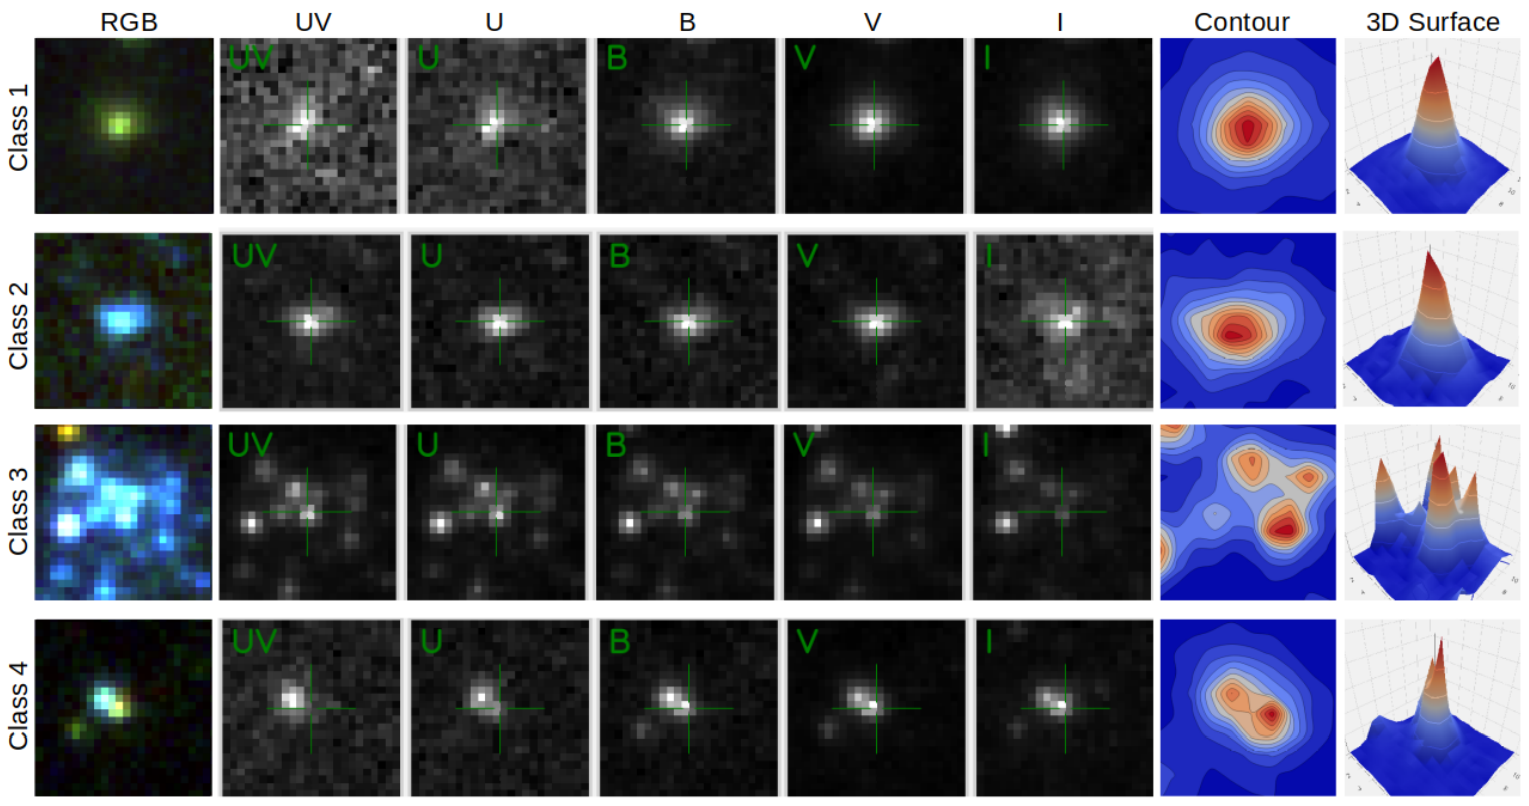
\includegraphics[width=9cm]{img/starcnet1.png} \pause

From \cite{perez_starcnet_2021}, LEGUS classification scheme. Examples of candidates from the LEGUS images of NGC 1566 classified as
Class 1 (symmetric star cluster; top), \pause Class 2 (elongated star cluster; middle-top), \pause Class 3 (compact, multi–peak association;
middle-bottom), and \pause Class 4 (spurious object; bottom). \pause The three–color image to the left is created using the NUV and U bands for the blue channel, the B band for green one, and the V and I bands for red one. The contour and 3D plots from the V–band are shown to the right of the figure.

\end{center}

\end{frame}

\begin{frame}{Star Cluster Identification}
 \pause
Convolutional Neural Network: \pause

\begin{center}

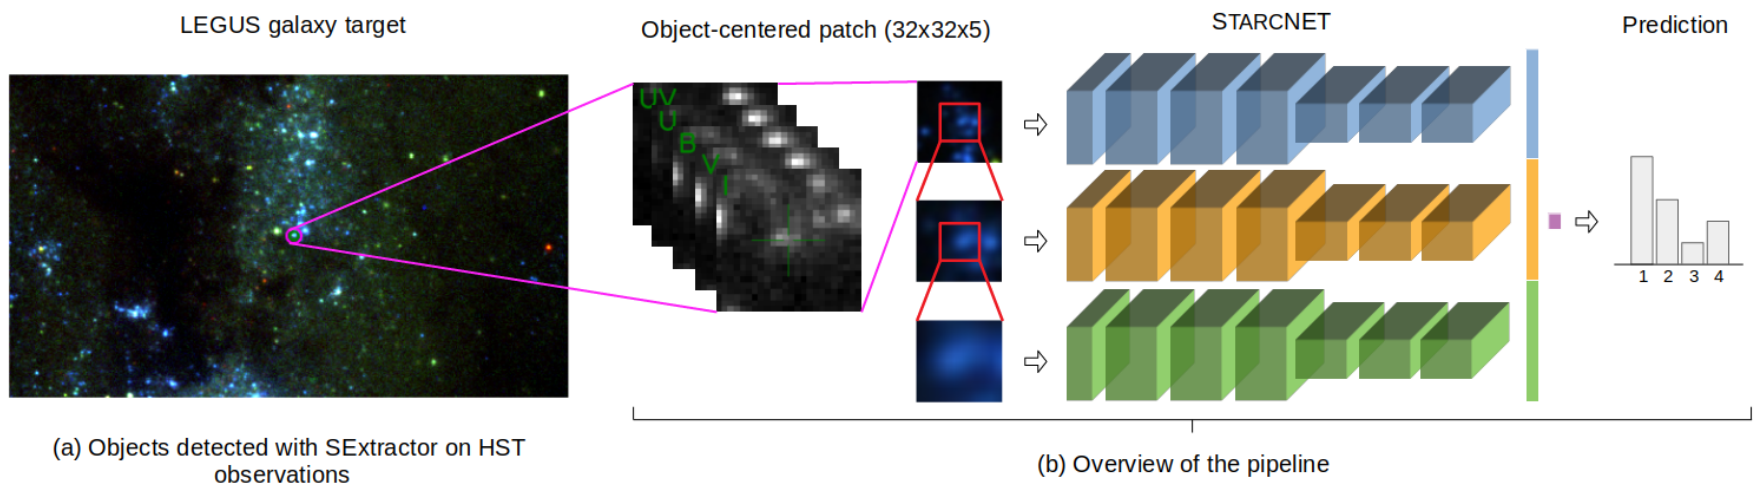
\includegraphics[width=11cm]{img/starcnet2.png} \pause

From \cite{perez_starcnet_2021}, the StarcNet pipeline. \pause Graphic sketch of the machine learning pipeline used in this work to classify cluster
candidates in the LEGUS images. \pause (Left): The Hubble Space Telescope images as processed by the LEGUS project through a custom pipeline to generate automatic catalogs of cluster candidates, which are part of the public LEGUS catalogs release (Calzetti et al. 2015; Adamo et al. 2017); we apply StarcNet to the LEGUS catalogs and images. 

\end{center}

\end{frame}

\begin{frame}{Star Cluster Identification}
 \pause
Convolutional Neural Network: \pause

\begin{center}

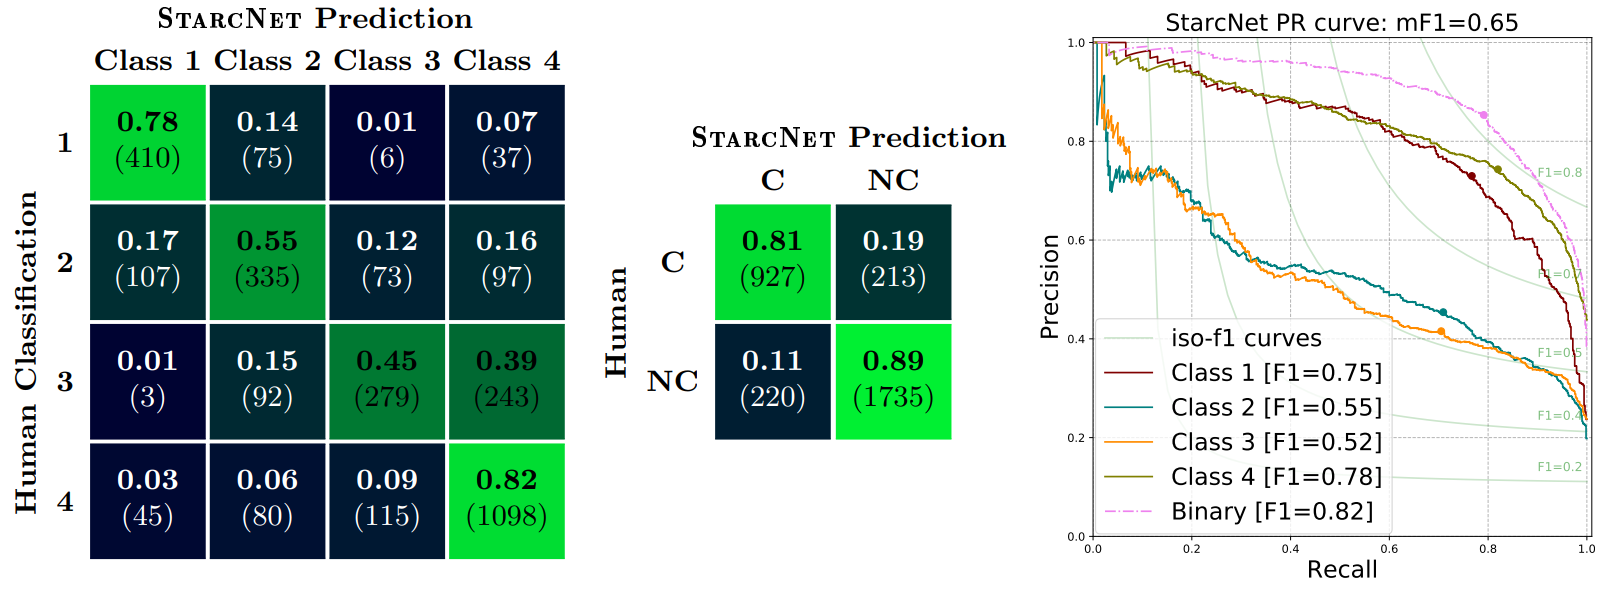
\includegraphics[width=9cm]{img/starcnet3.png} \pause

From \cite{perez_starcnet_2021}, performance of StarcNet on the test set. \pause Confusion matrix normalized over the classes in test set of the LEGUS dataset (20\% of the total sources or about 3000 objects). \pause The rows show the distribution of the human–classified sources, while the columns are the predictions of StarcNet. Parenthesis in the confusion matrix refers to the unnormalized values. \pause (Left) Overall accuracy evaluated for 4 class classification using raw bands as input. \pause (Middle) Results calculated with 2 classes (cluster/non-cluster classification). \pause (Right) Precision-recall curves for each of the four classes, as well as for binary classification. \pause The overall accuracy is 68.6\% with 4 classes and 86.0\% with binary classification.

\end{center}

\end{frame}

\begin{frame}{Optimal Transportation Star Cluster Identification}

Our method: \pause

\begin{algorithm}[H]
    Input: 
    
    $X$ : images $N \times m \times m$

    $\delta$ : noise level \pause

    Output:
    
    $C$ : star cluster classification $N \times 1$ \pause

	\For{$n=1,2,...,N$}
 	{
     	$ V_n = \arg\min_{v':d_W(X_n,v')<\delta} H(v')$ \pause
     	
        \eIf{ $rank(H_0(V_n^{-1}([0.9, 1]))) == 1$ }{ \pause
            $ C_n = 1 $
        }{
            $ C_n = 0 $
        }
  	}
	\caption{Optimal Transportation Star Cluster Identification}
\end{algorithm}

\end{frame}

\begin{frame}{Optimal Transportation Star Cluster Identification}

Evaluating the expression $\arg\min_{v':d_W(x,v')<\delta} H(v')$
\pause

Note: Center the problem at $x$ and add small vectors to stay in feasibility region. Normalize vectors to stay in probability space. \pause

\begin{enumerate}
    \item Uniform grid search: \pause
    
    \begin{enumerate}
        \item Converges first order (Taylors Remainder) \pause
        
        \item Computationally slow and exponentially slow in higher dimensions \pause
    \end{enumerate}
    
    \item Random search: \pause
    
    \begin{enumerate}
        \item Converges with high probability \pause
        
        \item Exponentially slow in higher dimensions \pause
    \end{enumerate}
    
    \item Gradient Descent: \pause
    
    \begin{enumerate}
        \item Converges quickly to local minimum (usually) \pause
        
        \item Misses global minimum and can even diverge
    \end{enumerate}
\end{enumerate}

\end{frame}

\begin{frame}{Optimal Transportation Star Cluster Identification}
Results:

Preliminary results on class 2 cluster detection: \pause

$precision = \frac{tp}{tp+fp} = 1$

$recall = \frac{tp}{tp+fn} = 2/5$

$F_1 = 2 \frac{precision \cdot recall}{precision + recall} = \frac{4}{7} = 57\%$\\~\\

\pause

Future Work: \pause
\begin{enumerate}
    \item Investigate transporting data across spectrum, not just spacially. \pause
    \item Estimate SNR parameter. \pause
    \item Speedup on GPU. 
\end{enumerate}

\end{frame}

\begin{frame}{Bibliography}
    
    \bibliographystyle{abbrv}
    \bibliography{ref}
    
\end{frame}

\end{document}

